\chapter{Testing}
\label{ch:testing}
Testing was an important part of the project. The application interface and the functionality were continuously tested throughout the development process. In addition to that, the most critical parts of its business logic were covered with unit tests.

On completion of the implementation phase, the System Integration Testing was carried out. During this testing process functions of the project were reviewed against the original specifications and any issues arising from this testing were noted. Also, the system was tested for its non-functional requirements, such as performance, responsiveness, cross-browser compatibility, etc.

Finally, the User Acceptance Testing was performed, making sure that the application works well for the intended end users. 

This chapter describes the testing carried out and the points raised by it.

\section{Unit Testing}
\label{sec:unittesting_test}
Unit testing is the practice of testing different elements of the software using a test program to provide inputs to each element and evaluate the outputs.
Known as white-box testing (meaning that the internal structure of the software is known to the tester), the tests are usually written before or at the same time as the tested componenents. According to Miguel Grindberg \citep{book:Grindberg2014FlaskWebDevelopment}, "There are two very good reasons for writing unit tests. When implementing new functionality, unit tests are used to confirm that the new code is working in the expected way. ... A second, more important reason is that each time the application is modified, all the unit tests built around it can be executed to ensure that there are no regressions  in the existing code; in other words, that the new changes did not affect the way the older code works." In a way, tests provide a safety net, meaning you can refactor the code at any time without the risk of breaking the original functionality.

Due to the time constraints, the focus was on testing only most critical parts of the project functionality. For this project it was especially important to ensure good code coverage for the business logic behind the model layer (prediction feature) and the external service layer of the application (api wrapper). This is explained in the chapter "Implementation" \ref{ch:implementation}, section "Application Architecture". SureThing has a suite of 30 unit tests that can be run anytime to validate this part of the application functionality. Tests in this project are performed using the Python \emph{unittest} library.

\begin{figure}[H]
	\begin{center}
		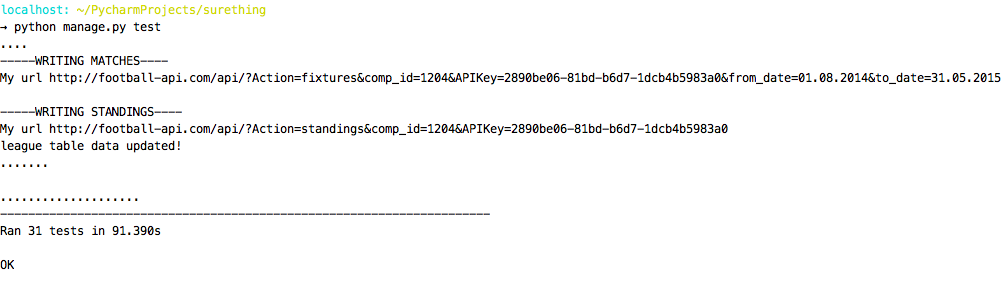
\includegraphics[width=.90\textwidth]{testing/images/unittestsOk}
		\caption{A screenshot of the terminal output showing the successfully passed test suite of the SureThing.}
		\label{fig:using:unitttestsok}
\end{center}
\end{figure}

\section{Continuous Integration with Travis CI}
\label{sec:travis_test}
As the application grows, it may begin to take too long to run the unit tests. Therefore, it is worth automating this process by setting up a "Continuous Integration" or CI server. Travis CI was chosen for this task because it is easy to set up and available for free as a part of the GitHub Student Developer Pack.
The service takes care of the unit testing allowing the developer to focus purely on the development process. Travis builds are triggered automatically when developer checks in the project code into the GitHub repository. Intergating Travis CI was just a matter of creation a configuration file \emph{travis.yml}.

\begin{figure}[H]
	\begin{center}
		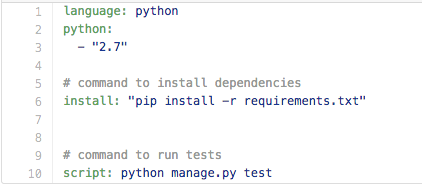
\includegraphics[width=.60\textwidth]{testing/images/travisYml}
		\caption{Travis CI configuration file.}
		\label{fig:using:travisyml}
\end{center}
\end{figure}
	
A Travis status icon indicating whether the tests passed or failed was embedded into the README file. This is a convenient feature that helped to keep an eye on the build status from the GitHub repository.

\begin{figure}[H]
	\begin{center}
		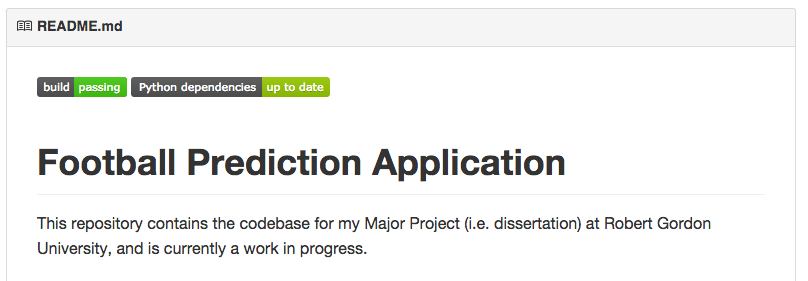
\includegraphics[width=.90\linewidth,natwidth=610,natheight=642]{testing/images/travisBadge}
		\caption{An extract from README on GitHub. Travis status icon indicates that the last build passed.}
		\label{fig:using:travisbadge}
	\end{center}
\end{figure}

\section{System Integration Testing}
\label{sec:systemintegration_test}
System testing is a black-box testing conducted on a finalised software, where its external workings are evaluated against a set of functional and non-functional requirements. The aim of this high-level testing is to find possible defects on different components of the system before the software release \citep{web:testingclass}. 

\subsection*{Functional Testing}
Functional Testing is concerned with the functional requirements of the developed system. It includes tests based on the initial specifications, use cases, or other high-level descriptions of the software behavior. The testing is performed by the developer, who takes into account the expected outputs and compares them with the actual result for each of the test cases.

For the purposes of System Testing, all the functionality of the application was reviewed against its initial specification and no major issues were discovered. The testing results can be found in the Appendix \ref{ch:requirementsreview_appendix}.

\subsection*{Non-Functional Testing}
In the final step of the System Testing, the readiness of a software was evaluated using the project non-functional requirements. The output of the testing can be found below. 

Usability - The application is extremely user friendly, it is uncluttered and navigation is highly intuitive. The initial test users praised the design and overall ease of use of the application.

Responsiveness - The responsiveness of the application was checked with the help of the Chrome "Window Resizer" extension. SureThing is a fully responsive website, tested successfully on a variety of screen resolutions down to a minimum of 640x960 (DVGA).

Performance - During the whole development process, the focus was on the performance of the application. It was important to make sure that the user does not have to wait too long for the page to load. Therefore, the loading time for each page was measured and evaluated. If the speed was too slow, the appropriate code optimisation was made to ensure the speed is at an acceptable level. At the moment the average load time for the main page and the list of matches saved to the dashboard is 4 seconds and 4.5 seconds for the upcoming match view. All other pages of the application load within 1 second. A Chrome extention "Page load time" was used to perform this testing.

Cross-browser support - The website was tested and works on all the usual web browsers including Chrome, Firefox, IE9 and Safari.

Maintainability - The code written for the website is clear and understandable.  There is no doubt that other developers would find it easy to see what has been done and why it was done a certain way.

Extensibility - It became clear early on that the application has the potential to be of a much larger scale.  With this in mind, the project was developed to make it a simple matter of adding new and advanced features to it without having to rewrite large parts of the code.


\section{User Acceptance Testing}
\label{sec:uat_test}
During the final stage of the project, the completed application was given to a selection of target users to perform User Acceptance Testing. This type of testing helps to verify that the final product is easy to understand and use and that it in general works well for the users. User Acceptance Testing or UAT is a black-box technique, meaning that the testers are not aware of the internal workings of the code. It is important that the end users are asked to perform tasks close to how the application would be used in real life.

A suite of test cases highlighting the key functionality of the designed software must be created to perform UAT. In order to test SureThing, the following set of cases were designed and presented to the end users (UAT testers), alongside a questionnaire that can be found in the Appendix \ref{sec:ua_questions_appendix}.

\begin{enumerate}
  \item Create a new account
  \item Login into the newly created account
  \item Look through the list of matches and choose the ones you are the most interested in, then save them to dashboard
  \item Set your own prediction weights
  \item Commit to betting on a match
\end{enumerate}

The raw data collected from the user acceptance testing can be found in the Appendix \ref{sec:ua_answers_appendix}.

A number of potential end users were asked to test the application using the above set of steps. It is possible to say that the testing was successfull and the application was well accepted by all the respondents. However, the aim of the UAT is to identify and resolve drawbacks in the tested software. The performed testing helped to find some issues with regards to the key functionality.

According to the feedback, the most difficult steps to carry out were "saving matches to the dashboard," "committing a match" and "setting own prediction weights". First of all, it looks like the application needs a better way to communicate, why a user needs to save a match to the dashboard before committing to bet. Secondly, SureThing offers two ways to preview an unplayed match and the user needs to "open" a saved match \emph{from the dashboard} in order to see all the prediction features, be able to adjust the prediction outcome and commit the match. This is a known issue and a suggested resolution would be to allow the user to see a match in the full "prediction mode" as soon as the match has been saved by the user.

Most of the users found that it easy to set up a new account (the average score was 8.7 out 10), they found it moderately easy (the average score was 6.8 out 10) to find and set the prediction settings and an large majority agreed that the website offers enough statistics to support their betting decision (6 out of 7 testers). An interesting point is that some users mentioned that it was not quite clear why they need to set a default set of prediction settings. The application clearly needs a tutorial or a FAQ page, that would explain the purpose of the different levels of settings.

When asked about the "worst aspects of the application", testers again mentioned the lack of an explanation of how prediction settings work and lack of different football leagues. The fact that only one league is supported at the moment is due to the fact that to have more would cost more money. If the application was to be expanded, this would be the one of the first extensions to be made. As to the "best aspects", many of the users praised the application for its neat design and simple layout. Most of them also mentioned that the way the stats are presented is very effective and relevant to the prediction feature.

In general, the User Acceptance Testing was very beneficial and provided a valuable feedback from the potential users. The first outcome is that the application needs a help page or a tutorial. The concept of the dashboard also needs to be revisited and possibly redesigned, as not all of the testers were clear of its purpose. Some of the answers were very inspirational in terms of the future development. For example, one of the respondents would like to see an option to compete against a team of friends and be able to see a separate leaderboard.

Due to the time constraints, the resolution of the findings is beyond the scope of this project but the testing certainly proved it's worth and for future development of the project this information is extremely useful.
